\section{BON extraction}
The \textsc{bon} extractor is a static analysis tool that allows the user to get an overview of a program written in Eiffel using EiffelStudio. Its purpose is to take use of the features of the \textsc{bon} language without having to leave an Eiffel development environment, and without having to write the textual \textsc{bon}.

\subsection{Overall architecture}
The \textsc{bon} extractor has two main parts. One is the interface for EiffelStudio; the other is the internal representation of the \textsc{bon} language. Each of the two parts are independent and changes can be done in one without it having any effect, with the exception of feature calls done from one to another. These, however, are few and far between. 

\paragraph{}
For generating textual \textsc{bon} syntax an internal representation of \textsc{bon} has been made. This representation has a MOG-like structure with classes representing most \textsc{bon} structures, with a few exceptions (See section \ref{deviations_from_bon}).  Each of these classes contains meta information about the structure, and knows how to format textual \textsc{bon} (both formal and informal) based on this information. 

\paragraph{}
The objective of the extractor is to build bridge between the Eiffel universe and the \textsc{bon} universe.  In this case EiffelStudio represents the Eiffel universe and the \textsc{bon} universe is represented by an internal \textsc{bon} object graph.
\begin{figure}[H]
\centering
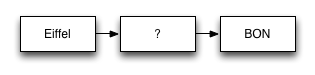
\includegraphics[scale=0.8]{images/BON-extraction-model-1.png}
\caption{BON Extraction Model 1}
\label{fig:bon_extraction_1}
\end{figure}

\subsubsection{From EiffelStudio to BON}
To create a bridge between EiffelStudio and the internal \textsc{bon} representation an interface that is linked with both parts is needed. It needs be able to take input from EiffelStudio, and hand over the abstract Eiffel syntax to the \textsc{bon} modeling section. In this implementation, it also takes care of knowing whether the current view is informal or formal \textsc{bon}. This could also be handled by the \textsc{bon} modeling section, but it will be discussed later, in the implementation section(See section \ref{why_interface_takes_care_of_formal_and_informal}), why this was not a practical solution.

\paragraph{}
With this interface there now is a link between Eiffel and \textsc{bon}, however the chain is not complete. There is still a missing link in making an internal representation of \textsc{bon} from the abstract syntax.
\begin{figure}[H]
\centering
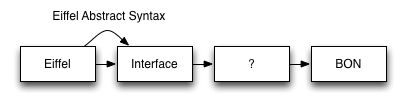
\includegraphics[scale=0.8]{images/BON-extraction-model-2.png}
\caption{BON Extraction Model 2}
\label{fig:bon_extraction_2}
\end{figure}

\paragraph{}
To create the \textsc{bon} representation a link (the missing link above) between the abstract syntax and the internal representation is needed. Making a meta-object that instantiates the modeling classes with basis in the abstract Eiffel syntax has done this. This meta-object will inspect the abstract Eiffel syntax and instantiate the \textsc{bon} objects based on the extracted information.
\begin{figure}[H]
\centering
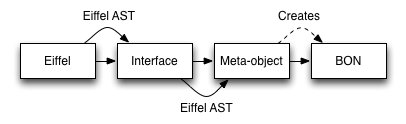
\includegraphics[scale=0.8]{images/BON-extraction-model-3.png}
\caption{BON Extraction Model 3}
\label{fig:bon_extraction_3}
\end{figure}

\paragraph{}
Since each of these \textsc{bon} objects knows how to generate textual \textsc{bon} syntax from the information given by the meta-object the system is now ready to generate \textsc{bon}. However, the textual \textsc{bon} still needs to be handed back to EiffelStudio for it to be viewed to the user.

\subsubsection{From BON to EiffelStudio}
Next step is for the modeling classes to hand back the formatted \textsc{bon} syntax to EiffelStudio for it to be shown to the user. To do this each previous step either needs a reference back to where the textual \textsc{bon} is needed, or to be able to receive the result of the following step and hand it back to its predecessor. In this implementation it has been decided to pass a reference back to the origin all the way to the \textsc{bon} representation, however it is transparent to the creator of the textual \textsc{bon} that it is writing directly to EiffelStudio.

\begin{figure}[H]
\centering
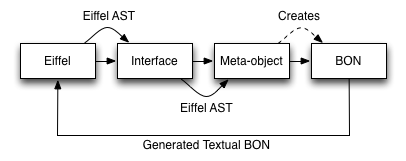
\includegraphics[scale=0.8]{images/BON-extraction-model-4.png}
\caption{BON Extraction Model 4}
\label{fig:bon_extraction_4}
\end{figure}

\subsubsection{Alternatives}
This way of extracting \textsc{bon} from Eiffel has the feel of a visitor pattern, but is not quite the same. This raises the question; why not use a visitor pattern? Had it been the intension to use the \textsc{bon} extractor for multiple languages a visitor pattern would have had its benefits, but since it is not the intension of the \textsc{bon} extractor to be used for any other language than Eiffel, a visitor pattern would only cause a more cluttered structure. Furthermore it would require all \textsc{bon} generation to be located in one class (the visitor class). This would lead to a confusing centralized structure and in the case of extending the \textsc{bon} generator would make it harder to locate where to extend the code. There would both be objects holding the data and representing the \textsc{bon} structure and be a central class taking care of handling the information.
\paragraph{}
An alternative solution would to only have one centralized class taking care of all the generation. This would require less overhead than the decided on solution, since it would remove the need for a meta-object and the need for the MOG-like representation of the \textsc{bon} grammar. This would however, like the visitor pattern, create a chaotic structure with all generation happening in a single class, and would make extension difficult. Furthermore, a procedural approach like this just does not feel in line with the object-oriented ideas involved in Eiffel and \textsc{bon}.

\subsection{Design decisions - Deviations from BON}
\label{deviations_from_bon}There are some deviations from the original \textsc{bon} grammar \cite[pp.~352-359]{walden1995}, both in the internal \textsc{bon} representation, but also in the generated textual \textsc{bon}. This section will discuss the most important ones, and attempt to justify their existence. 

\paragraph{}
The only major difference in in the generated \textsc{bon} is the omission of the \textit{Part} keyword. There are two uses of \textit{Part}. One is that one class in \textsc{bon} can exist over multiple documents. The extractor will never try and split a class up over more than one document, thus this use of  the keyword will not be needed. The other is the ability to have partial classes. This feature is seen in some languages (like C\#, \cite{msdn2009}), but since Eiffel does not support this there is no need for it in this implementation. Therefore the \textit{Part} keyword is not included in the generated \textsc{bon} nor modeled in the internal representation.

\paragraph{}
Lastly some elements such as Scenario\textunderscore chart and Creation\textunderscore chart are also not included. Some of these elements were excluded because they only hold semantic value and therefore require the static analysis to gather semantic information from the abstract syntax. Others have been excluded not because they did not feel relevant or useful for this tool, but because they felt out of scope. The \textsc{bon} extractor benefits more from analyzing specific classes and inheritance than from analyzing the relationship between them. This, however, does not mean that this is not something that could be included in the future.
